\documentclass[acmtog]{acmart}
% Title portion
\title{Project Impetus - Unity HLSL Real-Time rigidbody Solution} 
\author{Group Member:\quad Fang Zhixin, Diao Juanyu, Lu Yiren 
	}
\usepackage{graphicx}
\usepackage{listings}
\usepackage{hyperref}
% Document starts
\begin{document}
\maketitle

\vspace*{2 ex}


\section{Introduction}
\large
In this project, we implemented a GPGPU solution for rigidbody computation. The basis for GPU rigidbody simulation is to represent object by particles, and then handle the collision among those particles. We will focus on implementing particle collision rather than trying to represent object by particles, since our time is limited and we want to yield more attractive results.
This project will contain three parts:
\begin{enumerate}
	\item [1.] Rendering particles
	\item [2.] Improved GPU particle physics
	\item [3.] Inter-Particle collision detection
\end{enumerate}
An 3rd party library, Unity-CJ-Lib, is used. This lib contains basic quaternion/random utilities. It also has a ready-to-use GPU particle system, however it does not handle angular speed calculation as well as inter-particle collision. \\
\quad \\
\url{https://github.com/TheAllenChou/unity-cj-lib}\\
The version of Unity Engine is 2019 3.0f5, same as Unity-CJ-Lib.
\section{Implementation Details}
\subsection{Rendering Particles}
The strength of a commercial game engine is that it can do rendering with high level language, or even do it automatically. Unity-CJ-Lib provide an example of rendering particles, which can simply be done in one line of C\# code, and one very simple shader.
\begin{lstlisting}
Graphics.DrawMeshInstancedIndirect(m_mesh,
 0, m_material, 
 new Bounds(Vector3.zero, 20.0f * Vector3.one),
 m_instanceArgsBuffer, 0,
 m_materialProperties, 
 UnityEngine.Rendering.ShadowCastingMode.On);
\end{lstlisting}
This function draws instanced object with different parameters within the buffer. It consumes far less computational power than procedural mesh drawing because the GPU is in fact only drawing a same instanced object in parallel. In our case, \textbf{we can draw 10240 particles with 1000FPS on a GTX1060M laptop(without inter-particle collision).} 
\begin{figure}[!h]
	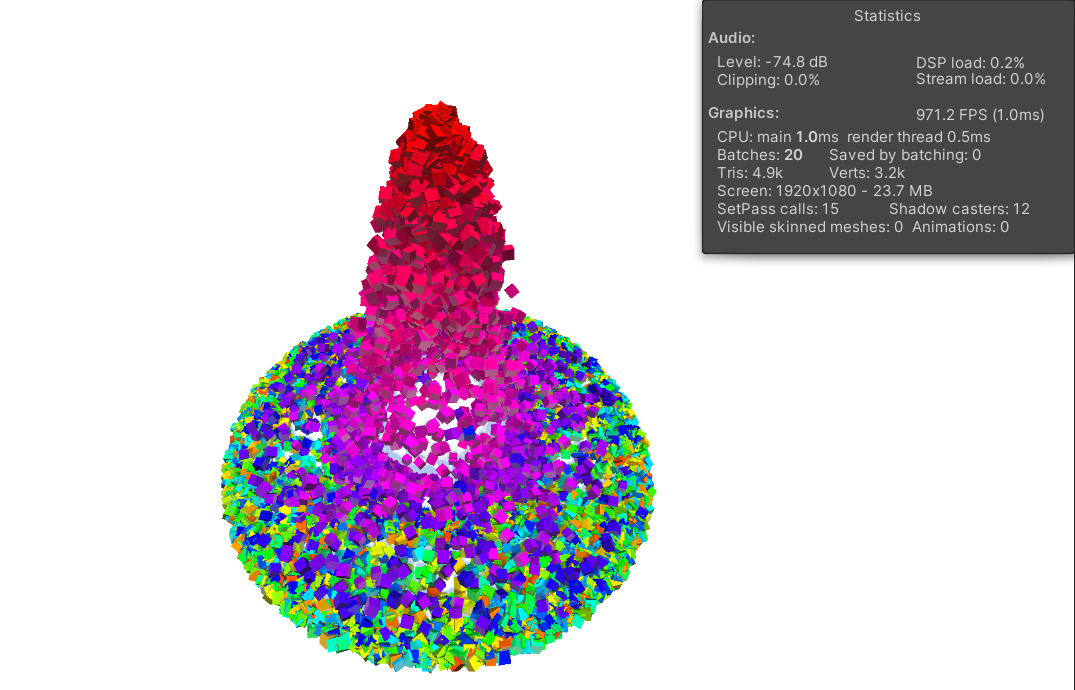
\includegraphics[width=\linewidth]{2-1-framerate}
	\caption{Collision with scene only, 10240 particles, 1920*1080 on GTX1060M}
\end{figure}
\subsection{Improved GPU Particle Physics}
This part is more of a preparation phase of the Inter-Particle collision detection. We test our physic models with simpler codes, let the particles collide with a single control ball in the scene to see the collision result.
To meet the requirement of general rigidbody physic calculation, we must implement GPU functions that handles both linear speed and angular speed.Two types of collision function are implemented - sphere(particle) versus sphere, and sphere versus plane.
\subsubsection{Representation of Objects}
\begin{enumerate}
	\item[] \textbf{Particles:} The particle can be regarded as a sphere in the space. To represent its position and movement, we store the position, scale, orientation(as quaternions), linear speed(as float3), angular speed(as quaternions) in the struct.
	\item[]  \textbf{Planes:} We'll need an efficient way to calculate the distance from the point to the plane later, hence the plane is represented as $Ax+ By+Cz+D = 0$, where $(A,B,C)$ is the normalized normal of the plane and D is calculated by a control point on the z axis.
\end{enumerate}
\subsubsection{Resolve Collision}
\quad \\
Generally, to resolve a collision we need the following information:
\begin{enumerate}
	\item [1.] Collision position(penetration distance) to determine the relative position of colliding objects.
	\item [2.] Relative linear speed.
	\item [3.] Relative angular speed. 
	\item [4.] Restitution factor, to determine how intense the particle will bump after collision.
	\item [5.] Friction factor, which affects the angular speed and the tangent linear speed.
	\item [6.] Collision normal vector.
\end{enumerate}
In this case we'll just assume that only the particle we're processing is spinning to simplify the problem. This should not cause problem in section 2.3 because we'll process every particle in fixed position in each frame.\\
\quad\\

\textbf{Algorithm for general collision calculation goes as follows:}\\
\subitem \underline{Linear Speed:}
\begin{enumerate}
	\item [1.] Orthogonal decompose the inbound speed. Compute the ratio of relative speed along the normal, representing the perpendicular impact force.
	\item [2.] Calculate friction force, proportional to the tangent speed and the perpendicular impact force.
	\item [3.] Calculate repulsive force, proportional to the velocity along the normal.
	\item [4.] Combine and calculate the force's effect on linear speed.
\end{enumerate}
\subitem \underline{Angular Speed:}
\begin{enumerate}
	\item [1.] Calculate a relative position vector(from mass center to contact point).
	\item [2.] Calculate the combined force on the object.
	\item [3.] Cross product the force and relative position, which is the torque caused by contact.
	\item [4.] Apply the torque on the object to get angular speed.
\end{enumerate}
Please note that in the actual implementation, many attribute of the object is omitted since we want to simplify the problem. We assume the mass of the particles is 1, and moment of inertia is 1 on all axis(since we only deal with balls).
\subsubsection{Sphere-Sphere Collision}
\quad \\
This part describes how to find attributes needed to resolve sphere-sphere collision in GPU.
\begin{enumerate}
	\item [1.] For collision position, simply get center difference between the two spheres. The sum of their radius - the length of difference is the penetration distance.
	\item [2.] Friction and restitution factor are passed as uniforms. More practically it should be store in the particle struct though.
	\item [3.] Dynamic parameters are stored in the particle struct. The relative speed can be calculated easily.
	\item [4.] Normal is always along the line segment connecting the two sphere centers. 
\end{enumerate}
\subsubsection{Sphere-Plane Collision}
\quad \\
The collision normal is obviously, the normal of the plane. The penetration distance can also be easily calculated if we know the distance from the sphere to the plane. Because we represent planes $in Ax+By+Cz+D = 0$ form, the distance can be directly obtained by substitute the position of the sphere in the equation.
\subsection{Inter-Particle Collision Detection}
Since there are hundreds of particles in the scene, it is impossible to traverse through each particle to calculate inter-particle collision velocity. This is some kind like calculate pixel intensity when it comes to ray tracing rendering. Thus, we use the same basic method as ray tracing: Grid. We assume the dimension of the overall grid is (64,64,64). It will be better if a flexible grid dimension is used. But to keep it simple, we use a fixed dimension.

\begin{enumerate}
	\item [1.] Calculate the unit grid size according to the particle numbers and active region size(calculated from the upper corner and lower corner) in the scene. The basic idea is that at most 4 particles will be in 1 grid in 1 frame. Use a one-dimensional array to store the grid structure. Each grid uses 4 slots storing the particle index to indicate which particles are in it.
	\item [2.] For each frame, first in GPU we reset all the variables in the grid array to particle numbers, meaning that all grids don't contain any particle. 
	\item [3.] Then in the GPU, we traverse every particle, calculate which grid they should be in, and judge the four slots in the grid. Store the particle index in the first slot that is not occupied yet. This is better done with atomic operation. We use interlock while writing into the grids.
	\item [4.] Next, in GPU, after we calculate particle collision situation with planes and control sphere, traverse the neighbor and self grid of each particle(27 grids in all) to calculate the inter-particle collision. calculate sphere vs sphere collision if there are any particles in those grids. 
	\item [5.] Finally, use the velocity of the particle we stored at the start of the frame, calculate the total delta velocity of the plane collision, sphere collision, and inter-particle collision. Add the delta velocity to the particle velocity so that it can be updated to a reasonable position. 
\end{enumerate}

\begin{figure}[!h]
	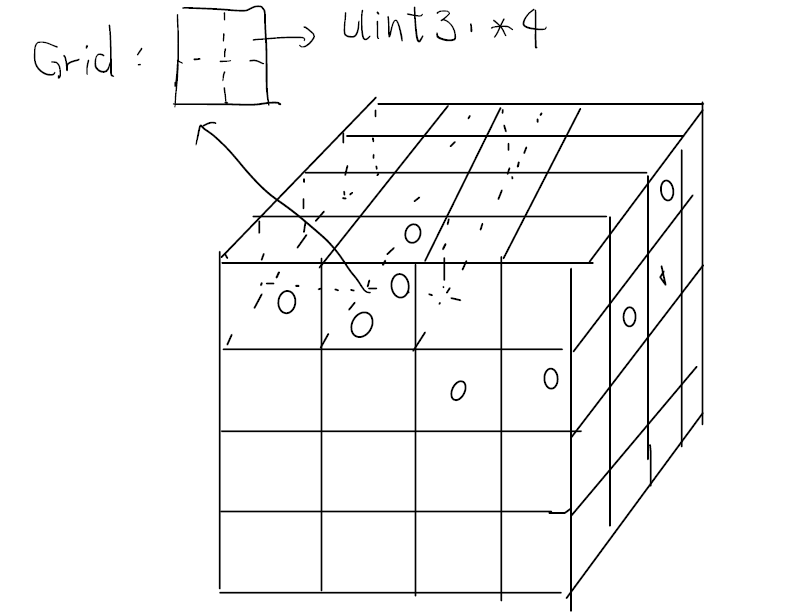
\includegraphics[width=7.2cm]{grid}
	\caption{Grid structure}
\end{figure}

\begin{figure}[!h]
	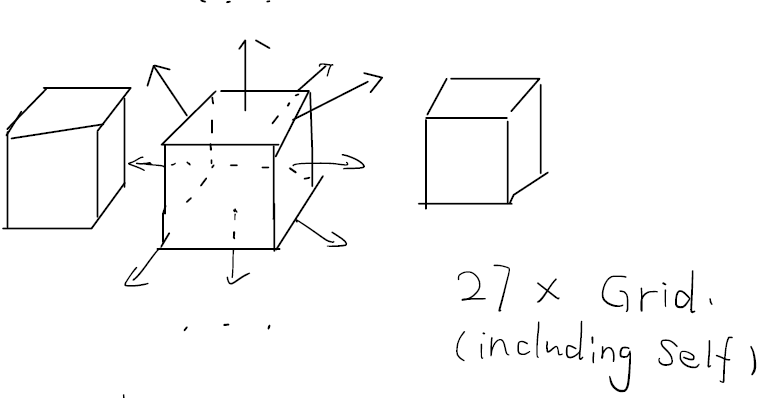
\includegraphics[width=6.1cm]{inter-particle}
	\caption{Inter-particle situation}
\end{figure}

\pagebreak
\quad \\

\pagebreak
\section{Results}
\begin{figure}[!h]
	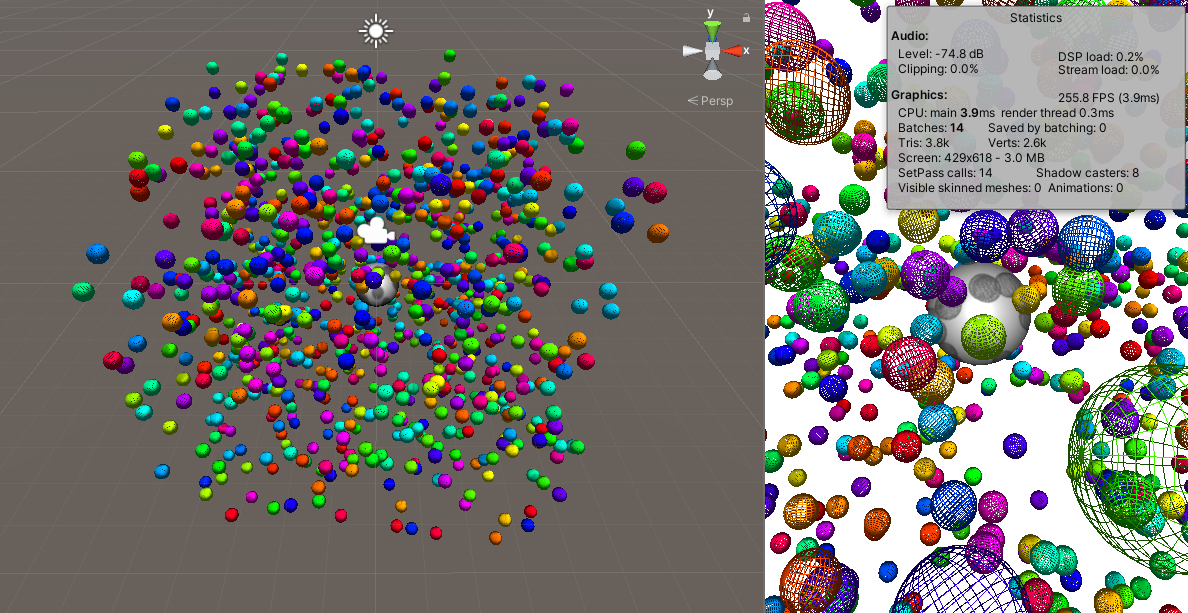
\includegraphics[width=\linewidth]{r1}
	\caption{Result of 1000 particles}
\end{figure}
\begin{figure}[!h]
	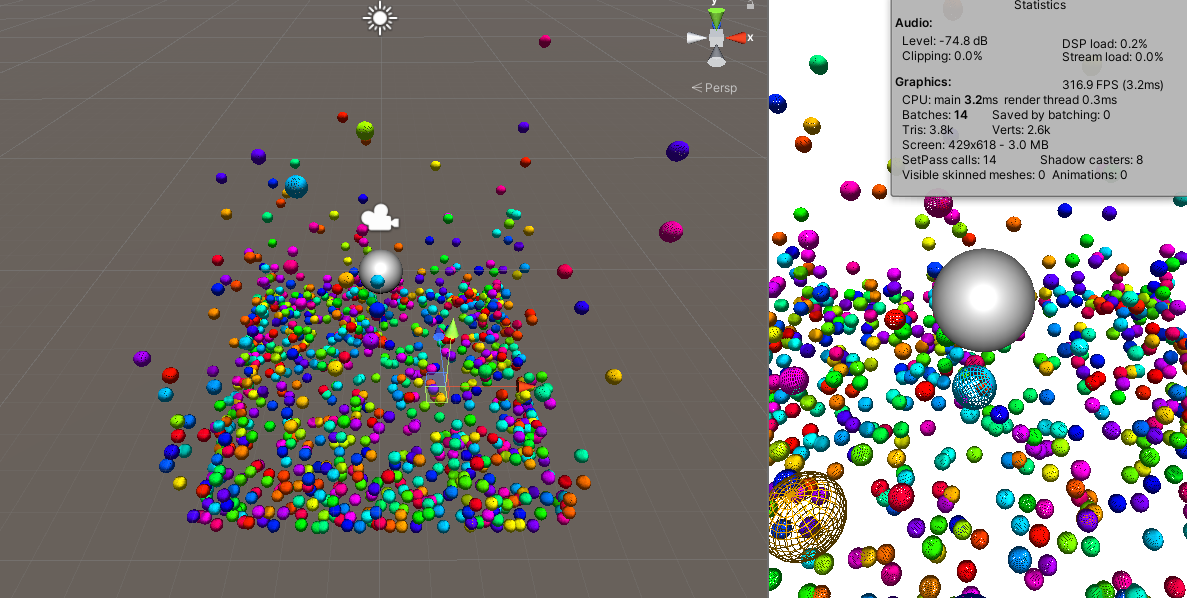
\includegraphics[width=\linewidth]{r2}
	\caption{Result of 1000 particles}
\end{figure}
\vspace{20mm}



\end{document}
